\section{Task Description}

A custom simulated environment has been created in order to test the algorithms and the exoskeleton. The simulated environment consists of UR5 robot equiped with robotiq 140 gripper, placed on a table Fig. \ref{fig:environment_setup}. The robot is initialized with the home pose of $\mathbf{q}_0 = \begin{bmatrix} -1.57 & -1.55 & 1.34 & -1.37 & -1.57 & 0 \end{bmatrix}^T$ at coordinates $(x, y, z) = (0, 0, 1)$. The position of the ball is initialized randomly by sampling from an uniform distribution Eq. \ref{eq:ball_init}.

\begin{align}
  \mathbf{p}_{\text{ball}} &\sim \text{Uniform}(\mathbf{p}_{\min}, \mathbf{p}_{\max}) \label{eq:ball_init} \\
  \mathbf{p}_{\min} &= \begin{bmatrix} -0.38 \\ -0.55 \\ 1 + r_{\text{ball}} \end{bmatrix}, \quad
  \mathbf{p}_{\max} = \begin{bmatrix} 0.38 \\ -0.38 \\ 1 + r_{\text{ball}} \end{bmatrix}
\end{align}

\begin{figure}[ht]
  \centering
  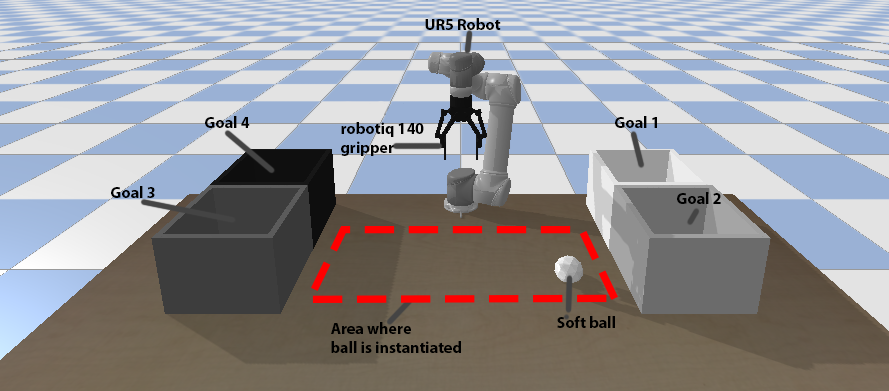
\includegraphics[width=1\textwidth]{chapters/algorithms/images/Environment_setup.png}
  \caption{Environment setup.}
  \label{fig:environment_setup}
\end{figure}

\noindent
During the initialization, the soft ball is assigned one of the four possible types Tab. \ref{tab:ball_classes}, the stiffness of each type varies based on the Young's Modulus. There are four boxes: $\mathbf{p}_{\text{goal},1} = (0.70, -0.16, 1), \mathbf{p}_{\text{goal},2} = (0.70, -0.50, 1), \mathbf{p}_{\text{goal},3} = (-0.70, -0.50, 1), \mathbf{p}_{\text{goal},4} = (-0.70, -0.16, 1)$. The boxes dimensions are 30x30x25cm and the walls are 2cm thick. The goal of the robot is to pick the ball and sort it according to it's type to the appropriate box. 

\begin{table}[ht]
  \centering
  \setlength{\tabcolsep}{6pt}
  \setlength{\abovecaptionskip}{6pt}
  \begin{tabular}{@{}cccc@{}}
      \toprule
      \textbf{Ball Type} & \textbf{Young's Modulus [min, max]} & \textbf{Density $(kg/m^3)$} & \textbf{Poisson's ratio} \\ 
      \midrule
      1 & [900, 1100] & 400 & 0.4 \\ 
      2 & [1400, 1600] & 400 & 0.4 \\ 
      3 & [1900, 2100] & 400 & 0.4 \\ 
      4 & [2400, 2600] & 400 & 0.4 \\ 
      \bottomrule
  \end{tabular}
  \caption{Ball types and their respective properties.}
  \label{tab:ball_classes}
\end{table}